\pdfoutput=1
\documentclass[3p,times,twocolumn]{elsarticle}

\usepackage[T1]{fontenc}
\usepackage{amsmath,amssymb,amsfonts}
\usepackage{booktabs}
\usepackage{graphicx}
\usepackage[hidelinks]{hyperref}
\usepackage{microtype}
\usepackage[section]{placeins}
\usepackage{siunitx}

\graphicspath{{figures_jcp/}}

\setlength{\textfloatsep}{10pt plus 2pt minus 2pt}
\setlength{\floatsep}{8pt plus 2pt minus 2pt}
\setlength{\dbltextfloatsep}{10pt plus 2pt minus 2pt}
\renewcommand{\topfraction}{0.9}
\renewcommand{\bottomfraction}{0.8}
\renewcommand{\textfraction}{0.07}
\renewcommand{\floatpagefraction}{0.85}
\renewcommand{\dbltopfraction}{0.9}
\renewcommand{\dblfloatpagefraction}{0.85}

\newcommand{\comm}[2]{[#1,\,#2]}
\newcommand{\tr}{\operatorname{Tr}}
\newcommand{\dv}[2]{\frac{d#1}{d#2}}

\journal{Journal of Computational Physics}
\biboptions{numbers,sort&compress}

\begin{document}

\begin{frontmatter}

\title{Hardware-Aware Performance Characterization of Small Dense Lindblad Propagation for Near-Term Quantum Control}

\author[erau]{Rylan Malarchick\corref{cor1}}
\ead{malarchr@my.erau.edu}
\cortext[cor1]{Corresponding author}

\affiliation[erau]{organization={Department of Engineering Physics, Embry-Riddle Aeronautical University},
             city={Daytona Beach},
             state={FL},
             postcode={32114},
             country={USA}}

\begin{abstract}
Dense Lindblad propagation at the Hilbert-space sizes most common in
near-term transmon control does not follow large-BLAS intuition. This paper
characterizes that regime on two x86 hosts (Intel Core i9-13980HX and AMD
Ryzen 5 1600), two NVIDIA GPUs (RTX 4070 Laptop GPU and GTX 1070 Ti), and a
Tang Nano 20K FPGA, using working-set analysis, empirical Roofline-style
summaries, and an end-to-end GRAPE-style benchmark against released QuTiP
5.2.3. The arithmetic intensity of the propagation kernel is low, but the
working sets at $d=3$, $9$, and $27$ are also small enough that cache
placement, launch overhead, and fixed latency determine which hardware is
actually useful. On CPU, OpenMP over independent batched states helps only
once the problem is large enough to amortize threading overhead: the i9
reaches 87.8 GFLOP/s at $d=9$ and 159.3 GFLOP/s at $d=27$, while the Ryzen
peaks at 58.7 and 47.2 GFLOP/s. For the measured CUDA kernel,
device-resident execution beats the best tested CPU at larger batches for
$d=9$ and $d=27$, but host-visible timing never crosses the CPU in the
measured range once packing, transfer, and launch costs are included. The
Tang Nano implementation targets only the $d=3$ kernel, but it executes in
95 cycles at 135 MHz (703.7 ns) with zero cycle-count spread over 500
trials, which places it in a deterministic-latency regime rather than a
throughput regime. The application result is more mixed than the kernel
result: after reusing invariant Lindbladian pieces and matrix-exponential
scratch in the C GRAPE benchmark, the C path is still 153--277$\times$
faster than released QuTiP 5.2.3 at $d=3$, and 1.9--4.1$\times$ faster at
$d=9$, but remains 4.0--4.3$\times$ slower at $d=27$ because propagator
construction dominates the total landscape-point cost. The main result is
that small dense Lindblad simulation splits into distinct CPU, GPU, and FPGA
operating regimes, and that end-to-end control performance is limited by
propagator construction before it is limited by propagation at the largest
tested size.
\end{abstract}

\begin{keyword}
Lindblad master equation \sep quantum optimal control \sep Roofline model
\sep GPU computing \sep FPGA acceleration \sep QuTiP
\end{keyword}

\end{frontmatter}

\section{Introduction}

The Lindblad master equation~\cite{Lindblad1976,Gorini1976} is the standard
Markovian model for open-quantum-system dynamics,
\begin{equation}
  \dv{\rho}{t} = -i\comm{H}{\rho}
  + \sum_k \left(L_k \rho L_k^\dagger
  - \tfrac{1}{2}\{L_k^\dagger L_k,\rho\}\right),
\end{equation}
and it appears in the main software loops of GRAPE, robustness studies, and
feedback-controller design for superconducting qubits~\cite{Khaneja2005}. In
the dense, time-independent case, vectorization turns one propagation step
into
\begin{equation}
  \vec{\rho}(t+\Delta t) = P\,\vec{\rho}(t), \qquad
  P = e^{\mathcal{L}\Delta t}, \qquad
  P \in \mathbb{C}^{d^2 \times d^2}.
\end{equation}
At $d=3$, $9$, and $27$, the hot path is a 9$\times$9, 81$\times$81, or
729$\times$729 dense complex matvec.

This size regime is awkward. It is too small to inherit classical large-BLAS
intuition, but too large for overheads to disappear. The asymptotic
arithmetic intensity of the propagation kernel approaches 0.5 FLOP/byte, so
a Roofline reading~\cite{Williams2009} says the kernel should live in the
bandwidth-sensitive part of the machine balance. In practice, however, the
relevant working sets are only about 1.5 KB, 105 KB, and 8.3 MB. That means
cache boundaries, kernel launch cost, and fixed-latency behavior matter as
much as nominal peak FLOP rate.

Existing Lindblad performance work has mostly gone in one of three
directions: general software frameworks such as QuTiP and its later
extensions~\cite{Johansson2012,Johansson2013,Lambert2026}, modern
accelerated or differentiable backends such as \texttt{qutip-jax},
\texttt{dynamiqs}, and adjacent JAX-based differential-equation software such
as Diffrax~\cite{QuTiPJax,Guilmin2024,Diffrax2026},
larger-scale parallel or algorithmic formulations~\cite{Meyerov2019}, or
hardware/control papers that assume the classical simulator as a given
rather than measuring it directly~\cite{Gebauer2020,Yang2021,Caune2024}.
What has been missing is a controlled comparison that asks the practical
question a software author actually needs answered: for small dense Lindblad
propagation, which hardware wins, under which timing model, and for what
notion of ``performance''?

That last point matters because isolated kernel speed is not the same thing
as end-to-end control speed. A GPU can win in device-resident timing and
still lose on wall clock because the problem is too small to hide launch and
transfer overhead. An FPGA can lose on throughput and still be the only
useful answer if the real constraint is deterministic embedded latency. A C
kernel can dominate QuTiP in propagation and still lose a GRAPE-style
application benchmark if propagator construction becomes the bottleneck.

This paper is therefore built as a comparison study. We combine a
roofline-guided working-set analysis with measurements on two x86 CPUs, two
GPUs, and a low-cost FPGA; we separate host-visible and kernel-only GPU
timing; we report deterministic FPGA cycle counts rather than USB wall time;
and we close with a GRAPE-style benchmark against released QuTiP 5.2.3. The
result is not a single universal winner. It is a map of operating regimes
for authors of quantum-control software.

\section{Problem Formulation and Measurement Protocol}

\subsection{Kernel and Working-Set Model}

Vectorizing $\rho$ gives
\begin{equation}
  \dv{\vec{\rho}}{t} = \mathcal{L}\,\vec{\rho},
\end{equation}
with $\mathcal{L}\in\mathbb{C}^{d^2\times d^2}$. Once the propagator
$P=e^{\mathcal{L}\Delta t}$ is built, the hot path is a dense complex
matvec. Counting a complex multiply-add as eight real floating-point
operations gives
\begin{equation}
  \mathrm{FLOPs} = 8d^4, \qquad
  \mathrm{bytes} = 16(d^4 + 2d^2),
\end{equation}
so the arithmetic intensity tends to 0.5 FLOP/byte from below. The hot
working set is the propagator plus one input and one output state vector in
double precision.

\begin{table}[t]
  \centering
  \caption{Problem sizes studied in this paper.}
  \label{tab:problem_sizes}
  \small
  \begin{tabular}{@{}rrrr@{}}
    \toprule
    $d$ & $d^2$ & hot working set & arithmetic intensity \\
    \midrule
    3 & 9 & 1.5 KB & 0.41 FLOP/byte \\
    9 & 81 & 105 KB & 0.49 FLOP/byte \\
    27 & 729 & 8.3 MB & 0.50 FLOP/byte \\
    \bottomrule
  \end{tabular}
\end{table}

\subsection{Implementations Compared}

The CPU baseline is a C11 library with dense Lindbladian construction, a
Pad\'e $[13/13]$ matrix exponential~\cite{Higham2005}, and several
propagation paths: scalar array-of-structures, compiler-auto-vectorized C,
explicit AVX2, and OpenMP over independent batched states. The local
i9-13980HX configuration used in this work exposed AVX2 but not AVX-512. In
other words, the measured Linux-visible ISA on the hybrid 8P+16E system was
AVX2-only rather than AVX-512-capable, which is consistent with the mixed
P-core/E-core configuration used on this SKU family. The measured comparison
is therefore scalar versus auto-vectorized versus AVX2 rather than an
AVX-512 study.

The CUDA comparison uses one thread per output row of the dense matvec and
reports two timing models: host-visible timing, which includes packing,
transfer, launch, and copy-back, and kernel-only timing with resident device
buffers. That separation is required here because the problem is small
enough that platform overhead can dominate device arithmetic.

The FPGA comparison targets only the $d=3$ kernel. The Tang Nano 20K design
implements a fixed-point 9$\times$9 complex matvec with UART control and an
on-chip cycle counter. The important metric is on-chip cycle-exact latency,
not USB-attached wall-clock time.

\subsection{Hardware and Fairness Choices}

The two x86 hosts were an Intel Core i9-13980HX laptop and an AMD Ryzen 5
1600 desktop. The i9 machine also hosted the RTX 4070 Laptop GPU. The Ryzen
desktop hosted the GTX 1070 Ti. The Tang Nano 20K board was attached to the
local machine for synthesis, flashing, and hardware timing.

All QuTiP timings use the pip-installable official release available during
benchmarking, \texttt{qutip==5.2.3}, installed under \texttt{uv}. The
current QuTiP documentation describes a matrix-form Lindblad path, but that
option was not available in the released 5.2.3 package installed on the
measured machines. The fair released baseline in this paper is therefore
default \texttt{mesolve}; if a later public release exposes that matrix-form
path, it should be treated as a separate baseline rather than folded into
the present results.

The main OpenMP sweep used \texttt{OMP\_PROC\_BIND=true} and
\texttt{OMP\_PLACES=cores}, but it did not use explicit \texttt{taskset} or
\texttt{numactl} pinning to force either the performance-core or
efficiency-core subset on the i9. An auxiliary scheduler-sensitivity check
with \texttt{taskset -c 0-15} (P-core set) and \texttt{taskset -c 16-31}
(E-core set) at batch size 128 found that E-core-only placement was
substantially weaker for the larger kernels, while the default scheduler
plus OpenMP core binding stayed within 4\% of explicit P-core-only
placement at $d=27$ and 16 threads. The reported i9 scaling curves are
therefore not pure P-core measurements, but their qualitative conclusions do
not depend on an unreported scheduling artifact.

\subsection{Reusable Propagator Construction for the GRAPE Benchmark}

The application benchmark models one GRAPE-like landscape point as a
piecewise-constant control sequence with segment-dependent drive amplitude.
This benchmark originally rebuilt the full Lindbladian and reallocated the
Pad\'e scratch stack for every segment. That was needlessly pessimistic.

For the current version, we split the generator into three reusable pieces:
the coherent static term, the coherent drive term, and the dissipative term,
so that each segment forms
\begin{equation}
  \mathcal{L}(\Omega_s) = \mathcal{L}_0 + \Omega_s \mathcal{L}_{\mathrm{drv}}
  + \mathcal{L}_{\mathrm{diss}}.
\end{equation}
We also added a reusable matrix-exponential workspace so repeated segment
exponentials stop reallocating large temporary matrices. Unit tests verify
that the decomposed superoperator construction matches the baseline
Lindbladian build, and that the workspace-backed propagator builder matches
the baseline propagator numerically.

\section{Results}

\subsection{Empirical Roofline Summary}

The empirical Roofline summary is easier to read as direct numbers because
the arithmetic intensities in Table~\ref{tab:problem_sizes} barely move
across $d=3$, $9$, and $27$. Table~\ref{tab:roofline_summary} therefore
reports the observed bandwidth ceiling, observed compute ceiling, and best
measured point at each $d$ for each platform in the same Roofline spirit as
Williams \textit{et al.}~\cite{Williams2009}. The CPU rows show the
cache-sensitive small-kernel regime directly. The GPU rows show the
resident-kernel opportunity directly, but only under kernel-only timing.

\begin{table*}[t]
  \centering
  \caption{Empirical Roofline summary expressed as direct numbers. Peak
  bandwidth and peak compute are the peak observed ceilings from the tested
  configuration grid on each platform. The $d=3$, $d=9$, and $d=27$ columns
  report the best measured point performance at fixed $d$. GPU rows use
  kernel-only timing.}
  \label{tab:roofline_summary}
  \small
  \resizebox{\textwidth}{!}{\begin{tabular}{@{}lrrrrr@{}}
\toprule
platform & peak bandwidth (GB/s) & peak compute (GFLOP/s) & $d=3$ point & $d=9$ point & $d=27$ point \\
\midrule
i9-13980HX & 319.5 & 159.3 & 14.5 & 87.8 & 159.3 \\
Ryzen 5 1600 & 120.3 & 58.7 & 26.2 & 58.7 & 47.2 \\
RTX 4070 (kernel-only) & 348.3 & 173.7 & 12.9 & 102.4 & 173.7 \\
GTX 1070 Ti (kernel-only) & 330.7 & 164.9 & 14.5 & 123.6 & 164.9 \\
\bottomrule
\end{tabular}
}
\end{table*}

The important difference is not a big change in arithmetic intensity; it is
the change in attainable ceiling. The dense matvec keeps roughly the same
intensity across the three problem sizes, but the attainable performance
still depends strongly on whether the working set is living in cache or
spilling deeper into the hierarchy. That is why the rest of the paper needs
more than one headline number.

\subsection{CPU: Threading Helps Only When Independent Work Exists}

The CPU result is not ``use all cores''; it is ``batch only when the work is
actually independent.'' At $d=3$, the working set is small enough that
single-state propagation is already cache-resident and OpenMP overhead hurts
more than it helps. The best measured single-state latencies were 309.5
ns/step on the i9 and 457.6 ns/step on the Ryzen.

That changes once the problem is large enough and the batch is large enough.
At batch size 128, the i9 reaches 87.8 GFLOP/s at $d=9$ and 159.3 GFLOP/s at
$d=27$. The Ryzen peaks at 58.7 and 47.2 GFLOP/s, respectively. The newer
Intel host benefits from a larger cache hierarchy and a stronger memory
system, while the older Ryzen still provides a useful lower-end x86 point.

\begin{figure*}[t]
  \centering
  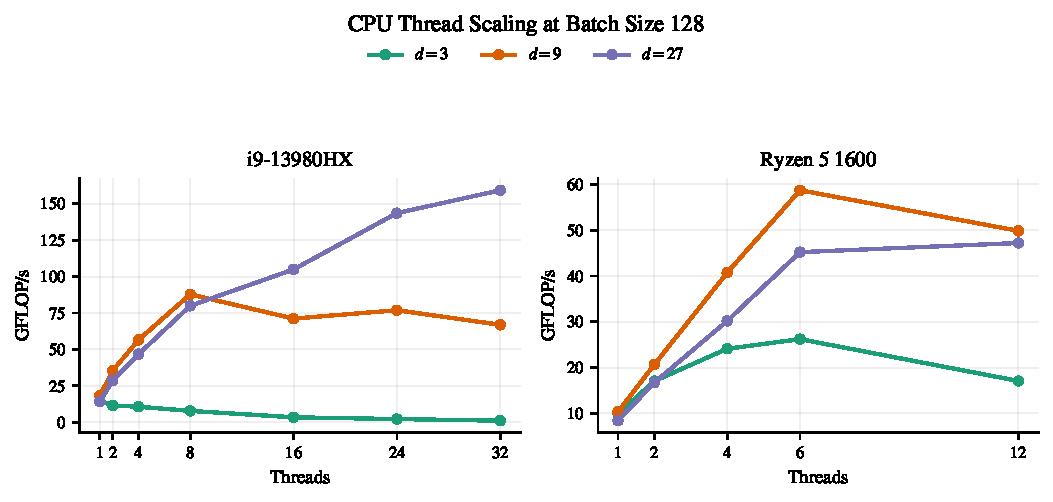
\includegraphics[width=\textwidth]{figure_cpu_thread_scaling.pdf}
  \caption{CPU thread scaling at batch size 128. Colors encode $d$ and the
  legend is shared across both panels. The important contrast is not between
  the two hosts alone, but between the three problem sizes. Threading does
  not help the tiny $d=3$ kernel, while $d=9$ and $d=27$ benefit once the
  batch is large enough to supply real parallel work.}
  \label{fig:cpu_threads}
\end{figure*}

\begin{table}[t]
  \centering
  \caption{Representative CPU summary. The $d=3$ entry uses the best measured
  single-state latency. The $d=9$ and $d=27$ entries use the peak measured
  throughput over the tested thread and batch grid.}
  \label{tab:cpu_summary}
  \small
  \resizebox{\columnwidth}{!}{\begin{tabular}{@{}lrrr@{}}
\toprule
host & $d=3$ latency (ns/step) & $d=9$ peak (GFLOP/s) & $d=27$ peak (GFLOP/s) \\
\midrule
i9-13980HX & 309.5 & 87.8 & 159.3 \\
Ryzen 5 1600 & 457.6 & 58.7 & 47.2 \\
\bottomrule
\end{tabular}
}
\end{table}

Figure~\ref{fig:cpu_threads} is the paper-safe thread-scaling statement. It
shows why parallel claims in this problem must be tied to independent batched
states rather than to the time steps of one trajectory. The data do not
support any broader claim than that.

\subsection{GPU: Kernel-Only Wins Appear Before Host-Visible Wins}

The GPU result is mixed in exactly the way small-kernel work tends to be
mixed. In the current CUDA implementation, host-visible timing never beats
the best tested CPU across the measured $(d,\mathrm{batch})$ grid. Kernel-only
timing does cross the CPU at larger batches for $d=9$ and $d=27$, which
means the missing wall-clock speedup is overhead, not device arithmetic.

This is also where the two GPU generations become interesting. The RTX 4070
does not simply dominate the GTX 1070 Ti at every operating point. For some
of the smaller kernel-only cases, especially at $d=9$, the older Pascal GPU
is still competitive or better in the current implementation. The RTX 4070
pulls ahead decisively only once the larger $d=27$, larger-batch operating
points begin to amortize the fixed costs.

\begin{figure*}[t]
  \centering
  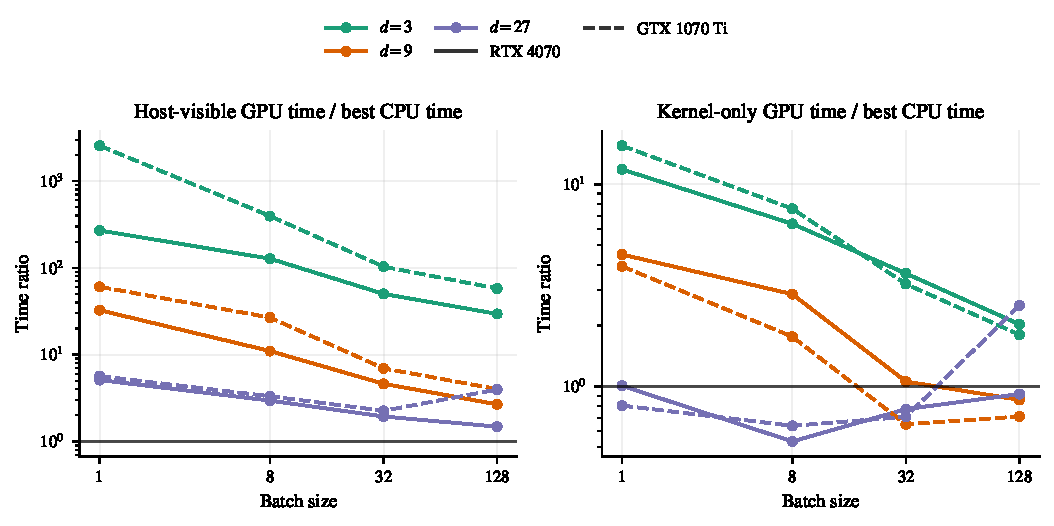
\includegraphics[width=\textwidth]{figure_gpu_cpu_ratio.pdf}
  \caption{GPU time normalized by the best tested CPU time at the same
  $(d,\mathrm{batch})$. Colors encode $d$ and line style encodes GPU model,
  with one legend shared across both panels. A value below 1 means the GPU
  is faster. Host-visible timing never crosses below 1 in the measured
  range. Kernel-only timing does, which shows that the device math can win
  before the full platform path does.}
  \label{fig:gpu_ratio}
\end{figure*}

Figure~\ref{fig:gpu_ratio} is the cleanest way to state the GPU result. The
host-visible panel never crosses 1. The kernel-only panel does. Any paper
claim that collapses those two timing models into one number would lose the
actual point of the measurement.

\subsection{FPGA: Deterministic Latency Rather Than Throughput}

The FPGA result is about deterministic latency, not throughput. The Tang Nano
section targets only $d=3$, but it contributes something the CPU and GPU
sections cannot. The programmed design ran at 135 MHz, used 1357 LUT4s and 4
DSP blocks, and matched the Python Q1.15 reference exactly over repeated
single-step and multi-step tests. The cycle counter measured a 95-cycle
single-step execution with zero spread over 500 trials. Multi-step timing
followed $94n+1$ cycles, which is consistent with a one-cycle command/setup
overhead around a 94-cycle steady-state matvec pipeline.

\begin{figure}[t]
  \centering
  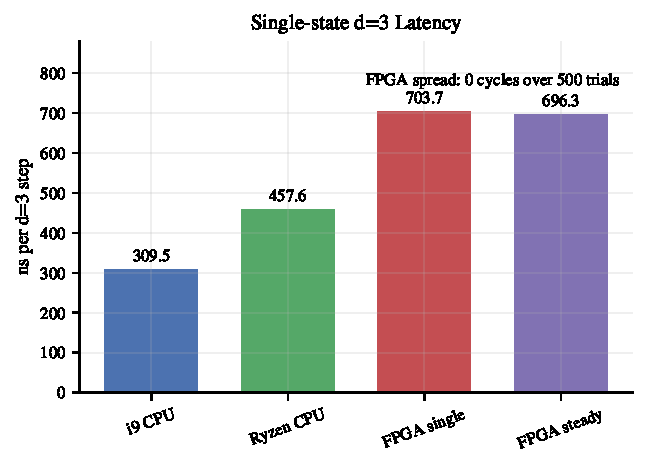
\includegraphics[width=\columnwidth]{figure_fpga_latency.pdf}
  \caption{Single-state $d=3$ latency comparison. The FPGA is not the latency
  winner against the tested CPUs, but it is the deterministic-latency
  winner: the measured single-step count had zero spread over 500 trials.}
  \label{fig:fpga_latency}
\end{figure}

\begin{table}[t]
  \centering
  \caption{Measured FPGA summary for the $d=3$ kernel.}
  \label{tab:fpga_summary}
  \small
  \resizebox{\columnwidth}{!}{\begin{tabular}{@{}lr@{}}
\toprule
quantity & value \\
\midrule
programmed clock & 135 MHz \\
single-step count & 95 cycles \\
single-step latency & 703.7 ns \\
long-run count & $94n + 1$ cycles \\
trial-to-trial spread & 0 cycles over 500 trials \\
LUT4 usage & 1357 / 20736 \\
DSP usage & 4 / 48 \\
\bottomrule
\end{tabular}
}
\end{table}

The important point is that this FPGA result is not a throughput result. The
best tested CPU single-state latencies at $d=3$ were still faster than the
FPGA, and the best batched CPU throughput was much faster. The value of the
FPGA is deterministic fixed latency inside hardware, not higher state-step
throughput. USB/UART wall time is milliseconds and is dominated by transport,
so it is not the number that belongs in the control discussion.

\subsection{Application Benchmark: Fast Propagation Does Not Guarantee Fast GRAPE}

Fast propagation does not guarantee fast GRAPE, and the $d=27$ case makes
that plain. After reusing invariant superoperator pieces and
matrix-exponential scratch, the C GRAPE benchmark became materially faster at
all three sizes. At $d=3$, the C path is now 153$\times$ faster than
released QuTiP 5.2.3 on the i9 and 277$\times$ faster on the Ryzen. At
$d=9$, the C path still wins on both hosts, by 1.9$\times$ on the i9 and
4.1$\times$ on the Ryzen. At $d=27$, however, QuTiP still wins by about
4$\times$ on both hosts.

\begin{figure}[t]
  \centering
  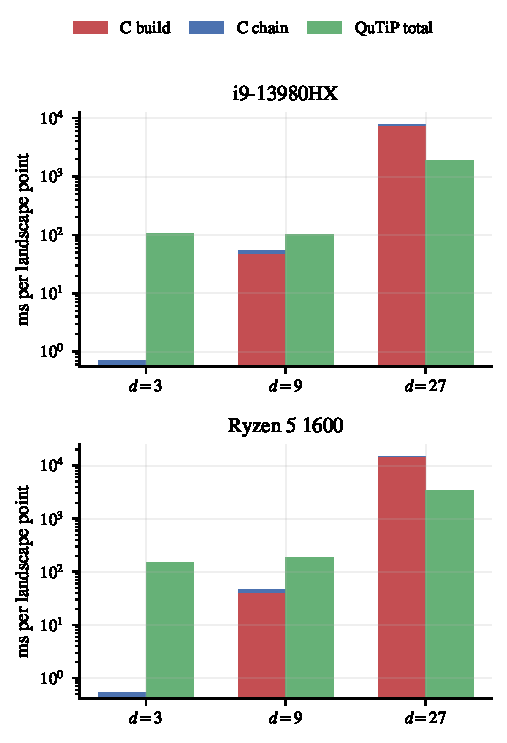
\includegraphics[width=\columnwidth]{figure_grape_breakdown.pdf}
  \caption{GRAPE-style landscape-point cost. The C path is separated into
  propagator construction and propagation chaining. The sign change at
  $d=27$ is not a contradiction of the propagation-kernel result; it shows
  that propagator construction becomes the dominant term once the generator
  is large enough.}
  \label{fig:grape_breakdown}
\end{figure}

\begin{table}[t]
  \centering
  \caption{End-to-end GRAPE-style benchmark using the optimized C benchmark
  and released QuTiP 5.2.3.}
  \label{tab:grape_summary}
  \scriptsize
  \resizebox{\columnwidth}{!}{\begin{tabular}{@{}llrrl@{}}
\toprule
host & $d$ & C (ms) & QuTiP (ms) & winner \\
\midrule
i9 & $d=3$ & 0.700 & 107.388 & C ($153\times$) \\
i9 & $d=9$ & 54.561 & 101.792 & C ($1.9\times$) \\
i9 & $d=27$ & 7697.947 & 1903.071 & QuTiP ($4.0\times$) \\
Ryzen & $d=3$ & 0.537 & 148.607 & C ($277\times$) \\
Ryzen & $d=9$ & 46.338 & 189.568 & C ($4.1\times$) \\
Ryzen & $d=27$ & 14724.661 & 3457.720 & QuTiP ($4.3\times$) \\
\bottomrule
\end{tabular}
}
\end{table}

Figure~\ref{fig:grape_breakdown} shows why. The propagation chain itself is
not the problem at $d=27$; the problem is that dense propagator construction
still dominates the landscape-point cost. This is exactly why the application
section needed to exist. A paper built only around propagation speedup would
have told an incomplete story. The current C implementation has a real kernel
advantage, a real application advantage at $d=3$ and $d=9$, and a real
application deficit at $d=27$. All three of those facts belong in the same
paper.

\FloatBarrier
\section{Discussion}

Three operating regimes emerge from the measured data.

First, CPU execution is the correct default for tiny dense work and for any
control loop where the available parallelism is limited. The CPU does not
win here because it has the highest theoretical peak. It wins because the
problem is small enough that low overhead and cache residency matter more
than raw peak arithmetic.

Second, the GPU story depends on which timing question is being asked. If the
question is whether a resident device kernel can outrun the CPU once there is
enough batched work, the answer is yes for the larger measured cases. If the
question is whether the full host-visible platform path already beats the CPU
in the measured range, the answer is no. Those are different claims, and the
paper should keep them separate.

Third, the FPGA occupies a different corner of the design space. It is not a
throughput replacement for CPU simulation. It is a deterministic-latency
result for an embedded control path. That distinction matters for
superconducting-qubit feedback electronics, where fixed response and jitter
can matter as much as bulk throughput~\cite{Gebauer2020,Yang2021,Caune2024}.

The GRAPE benchmark then gives the practical recommendation. For the current
code base, the next useful optimization target at $d=27$ is not another
round of propagation-loop tuning. It is propagator construction. That is the
term that still controls the end-to-end application cost once the propagation
kernel itself has been pushed into a good regime.

The obvious next methods step is therefore not simply ``more SIMD.'' It is to
push the control-affine reuse farther than the current benchmark already
does. This matters because the $d=27$ loss appears in repeated segment-wise
propagator construction, not in the propagation chain itself. The most
natural follow-on is therefore to reuse more of the update around
$\mathcal{L} = \mathcal{L}_0 + \Omega \mathcal{L}_{\mathrm{drv}} +
\mathcal{L}_{\mathrm{diss}}$, so closely related controls stop paying for a
near-full dense rebuild at every segment. If that still leaves too much
construction cost, then applying $e^{\mathcal{L}\Delta t}$ directly to the
state vector with a Krylov or Arnoldi method is the clearest algorithmic
break with the current dense-propagator path. The present measurements do
not choose between those two directions, but they do isolate the term that a
follow-on algorithmic study would need to reduce.

\FloatBarrier
\section{Conclusion}

This study measured small dense Lindblad propagation where near-term quantum
control software actually lives: not in asymptotic large-matrix HPC, but in a
size regime where cache placement, launch overhead, and deterministic latency
change the answer. The results split into clear operating regimes.

CPU execution is best for very small low-overhead work and remains the most
robust default. GPU execution can beat the CPU in kernel-only timing before
it beats the CPU in host-visible timing, so both timing models are required.
The Tang Nano FPGA establishes a deterministic-latency $d=3$ operating point
with 95-cycle single-shot execution and zero measured spread, but it is not a
throughput winner. At the application level, the optimized C GRAPE benchmark
wins decisively at $d=3$, still wins at $d=9$, and still loses at $d=27$
because propagator construction has become the leading cost.

The practical conclusion is therefore not a single hardware recommendation.
It is a division of labor: CPU for tiny dense work and low overhead, GPU for
sufficiently batched propagation once host costs are amortized, and FPGA for
deterministic embedded latency. For larger control problems in this
framework, the next method step is to reduce propagator-construction cost
rather than to keep optimizing propagation in isolation.

\section*{Data and Code Availability}

All benchmark code, raw timing data, figure-generation scripts, and
manuscript sources used in this study are available in the
\texttt{lindblad-bench} repository at
\url{https://github.com/rylanmalarchick/lindblad-bench}. It also contains the
CSV and log artifacts used to generate the reported tables and figures.

\section*{Declaration of Generative AI and AI-Assisted Technologies in the Writing Process}

OpenAI Codex and Anthropic Claude Code were used to assist with software
development, benchmark automation, figure-generation scripts, and language
editing. The author reviewed and edited all generated material and takes full
responsibility for the content of the publication.

\bibliographystyle{elsarticle-num}
\bibliography{refs}

\end{document}
